\let\negmedspace\undefined
\let\negthickspace\undefined
\documentclass[journal]{IEEEtran}
\usepackage[a5paper, margin=10mm, onecolumn]{geometry}
\usepackage{tfrupee} % Include tfrupee package

\setlength{\headheight}{1cm} % Set the height of the header box
\setlength{\headsep}{0mm}     % Set the distance between the header box and the top of the text

\usepackage{cite}
\usepackage{amsmath,amssymb,amsfonts,amsthm}
\usepackage{graphicx}
\usepackage{textcomp}
\usepackage{xcolor}
\usepackage{listings}
\usepackage{enumitem}
\usepackage{mathtools}
\usepackage{gensymb}
\usepackage{comment}
\usepackage[breaklinks=true]{hyperref}
\usepackage{circuitikz}

\begin{document}

\bibliographystyle{IEEEtran}
\vspace{3cm}

\title{11.16.3.5.2}
\author{EE24BTECH11066 - YERRA AKHILESH}

{\let\newpage\relax\maketitle}

\renewcommand{\thetable}{\arabic{table}}
\setcounter{figure}{0} % Ensuring figure numbering starts from 1
\setcounter{table}{0} % Ensuring table numbering starts from 1

\textbf{Question}:\

A fair coin with 1 marked on one face and 6 on the other and a fair die are both tossed. Find the probability that the sum of numbers that turn up is 12.\

\textbf{Solution: }\\
\textbf{Textual solution: }\\
The probability of a given event $A$ (where $A$: Sum of the numbers is 12) is computed using the independence of the coin and the die. Since these are independent events, we calculate their probabilities separately and then multiply them.

The probability of the coin showing 6 is:
\begin{align}
P_{X}(6) &= \frac{1}{2}
\end{align}
The probability of the die showing 6 is:
\begin{align}
P_{Y}(6) &= \frac{1}{6}
\end{align}
Since the events are independent, the probability of both occurring is:
\begin{align}
P(A) &= P_{X}(6) \cdot P_{Y}(6) = \frac{1}{2} \times \frac{1}{6} = \frac{1}{12}.
\end{align}

\textbf{Computational Solution:}

\subsection*{Probability Mass Function (PMF)}
The PMF, denoted as $P_Z(k)$, represents the probability of obtaining a sum $k$ in the sample space of $Z = X + Y$, where:
\begin{align}
X &\in \{1, 6\}, \quad Y \in \{1, 2, 3, 4, 5, 6\}.
\end{align}
The combined sample space is:
\begin{align}
S = \{(x, y) \mid x \in \{1, 6\}, y \in \{1, 2, 3, 4, 5, 6\}\},
\end{align}
with $|S| = 12$ total outcomes.

The PMF is then given by:
\begin{align}
    P_Z(k) &=
    \begin{cases}
        \frac{1}{12}, & k \in \{2, 3, 4, 5, 6, 8, 9, 10, 11, 12\}, \\
        \frac{1}{6}, & k = 7, \\
        0, & \text{otherwise}.
    \end{cases}
\end{align}

\subsection*{Cumulative Distribution Function (CDF)}
The CDF, $F_Z(k)$, represents the cumulative probability up to a given value $k$:
\begin{align}
F_Z(k) &= P(Z \leq k) = \sum_{j=2}^{k} P_Z(j),
\end{align}
where $k \in \{2, 3, \dots, 12\}$, and beyond $k = 12$, the CDF is 1:
\begin{align}
F_Z(k) =
\begin{cases} 
0, & k < 2, \\
\sum_{j=2}^{k} P_Z(j), & 2 \leq k \leq 12, \\
1, & k > 12.
\end{cases}
\end{align}

\subsection*{Z-transform Representation}
The Z-transform provides an analytical tool to compute the PMF for discrete random variables. It is defined as:
\begin{align}
M_Z(z) &= \sum_{k=2}^{12} P_Z(k) z^{-k},
\end{align}
where $M_Z(z)$ is the generating function for $P_Z(k)$.

\subsection*{Computational Process}
For the coin toss ($X$):
\begin{align}
P_X(k) &= \begin{cases} 
\frac{1}{2}, & k \in \{1, 6\}, \\
0, & \text{otherwise}.
\end{cases}
\end{align}
For the die roll ($Y$):
\begin{align}
P_Y(k) &= \begin{cases} 
\frac{1}{6}, & k \in \{1, 2, 3, 4, 5, 6\}, \\
0, & \text{otherwise}.
\end{cases}
\end{align}
The Z-transform for $X$ and $Y$ is:
\begin{align}
M_X(z) &= \frac{1}{2} z^{-1} + \frac{1}{2} z^{-6},
\end{align}
\begin{align}
M_Y(z) &= \frac{1}{6} (z^{-1} + z^{-2} + z^{-3} + z^{-4} + z^{-5} + z^{-6}).
\end{align}
The Z-transform of $Z = X + Y$ is given by:
\begin{align}
M_Z(z) &= M_X(z) M_Y(z).
\end{align}
Substituting:
\begin{align}
M_Z(z) &= \frac{1}{12} \sum_{k=2, k \neq 7}^{12} z^{-k} + \frac{1}{6} z^{-7}.
\end{align}

\textbf{Simulation:} \\
\begin{enumerate}
    \item Generate a random number for the coin toss using the \textbf{rand()} function.
    \item Restrict the random number to either $1$ or $6$ using \textbf{rand()} \% 2 and assign it to \textbf{coin}.
    \item Generate a random number for the die roll using \textbf{rand()} \% 6 + 1, and assign it to \textbf{die}.
    \item Compute the sum $\vec{Z} = \vec{X} + \vec{Y}$.
    \item Count occurrences where $\vec{Z} = 12$ over many trials.
    \item Estimate probability as occurrences divided by trials.
\end{enumerate}

\begin{figure}[ht]
\centering
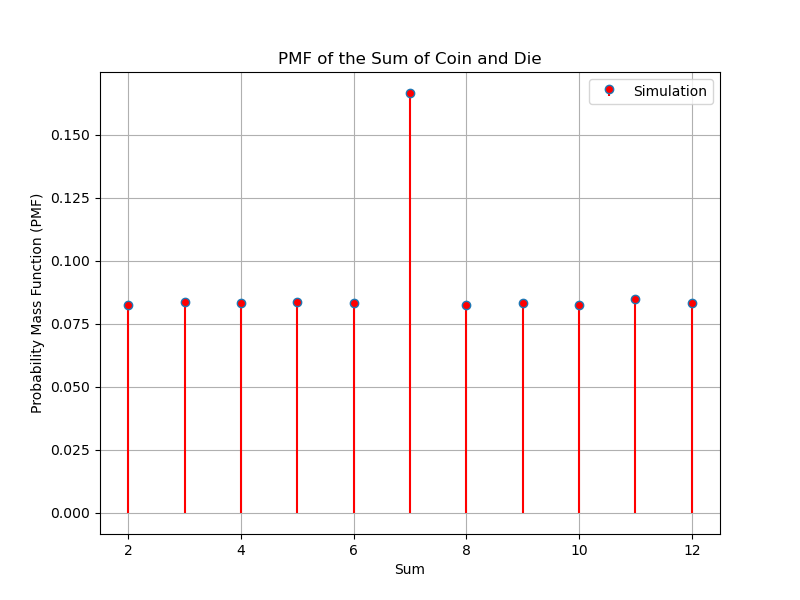
\includegraphics[width=\columnwidth]{figs/pmf.png}
\label{fig:pmf} 
\end{figure}

\begin{figure}[ht]
\centering
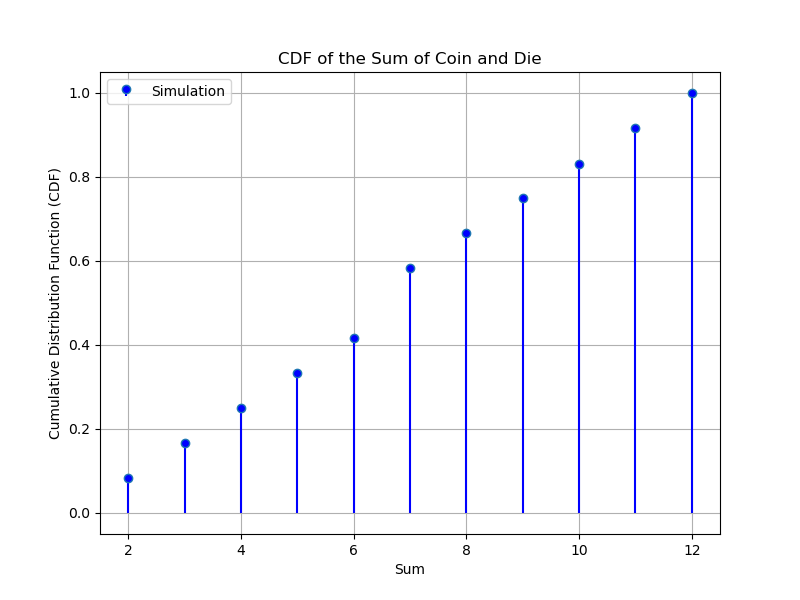
\includegraphics[width=\columnwidth]{figs/cdf.png}
\label{fig:cdf} 
\end{figure}

\end{document}

